


\begin{frame}{Title \sof{1}{2}}

%\vspace{1em}
\justifying

Foo

\vspace{2em}

% \twocol{0.5}{
% \justifying
% Our technical report~\cite{Dahm2004} provides an in-depth look into the core
% challenges of teaching robots to play soccer, the solutions developed by our
% team, and the involved support infrastructure. 

% \vspace{1em}
% As part of the GermanTeam -- a collaboration between the universities of Berlin,
% Bremen, Darmstadt, and Dortmund -- we won the world championship in the SPL 
% as well as the SPL Open Challenge.

% }{0.41}{
% \vspace{-1.75em}
% \begin{figure}
% 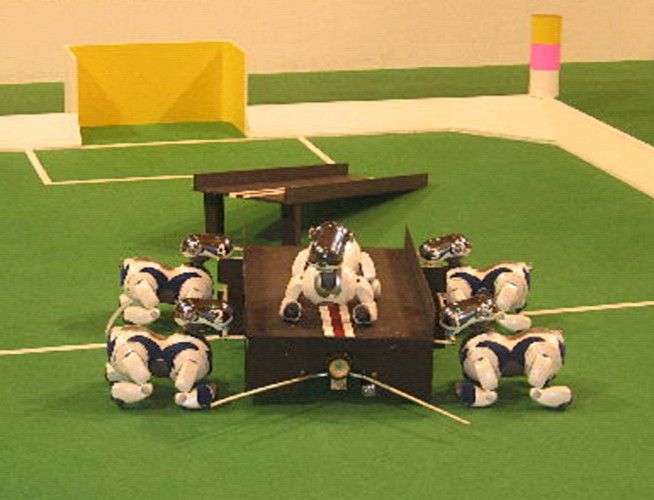
\includegraphics[width=\linewidth]{robocup/robocup.jpg}

% \vspace{-1em}
% \caption{\scriptsize Scene from the SPL Open Challenge~\cite{Dahm2004}.}
% \end{figure}
% }

\vspace{1em}

\begin{center}
\rule{2cm}{0.4pt}\\[0.5em]
\end{center}

\fc{kerdels2013b}{publications/2013-01/2013-01}\nombestpaper\\[1em]
\fc{kerdels2015b}{publications/2015-01/2015-01}\\[1em]
\fc{Kerdels2016}{publications/2016-01/2016-01}\\[1em]
\fc{Kerdels2016a}{publications/2016-03/2016-03}\bestpaper\\[1em]
\fc{Kerdels2016c}{publications/2016-04/2016-04}\nombestpaper\\[1em]
\fc{kerdels2017}{publications/2017-01/2017-01}\\[1em]
\fc{Kerdels2018b}{publications/2018-02/2018-02}\\[1em]
\fc{Kerdels2019}{publications/2019-02/2019-02}\\[1em]
\fc{Kerdels2019a}{publications/2019-01/2019-01}

\end{frame}
